% fig3-breakeven.tex
% Decision-rule break-even curve with measured sections overlaid.
% x-axis  = access frequency f in [0,1]
% y-axis  = f * r / |s|  (dimensionless ratio; 1 when r ≈ |s|)
% Break-even line: y = 0.235  (ρ=0.85, α=0.10 from Eq. 3)
%
% Frequency estimates per section (added here per TRIM-05 brief, not in CSV):
%   must-resident sections:      f ≈ 0.80–1.00
%   freq-deciding (kept):        f ≈ 0.35
%   freq-deciding (externalised):f ≈ 0.20
%   redundant:                   f ≈ 0.05
% r/|s| ≈ 1 (on-demand read cost ≈ section token count).

\begin{figure}[ht]
\centering
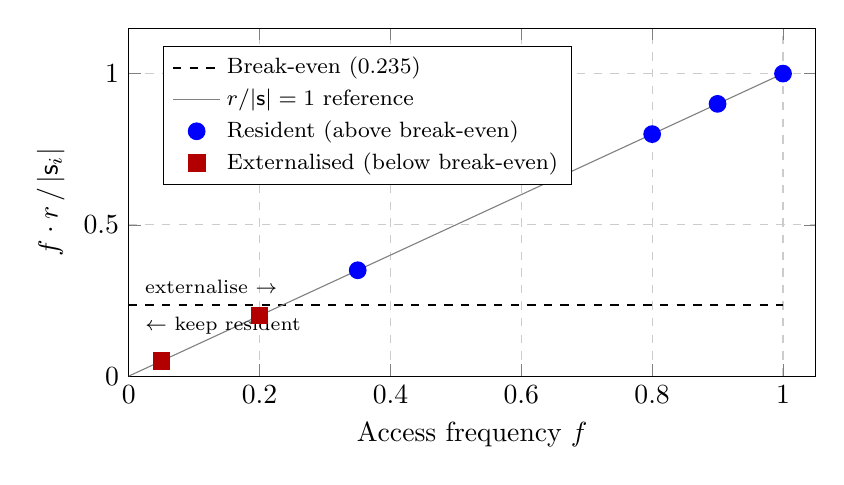
\begin{tikzpicture}
\begin{axis}[
  width=0.85\textwidth,
  height=6cm,
  xlabel={Access frequency $f$},
  ylabel={$f \cdot r \,/\, |\mathsf{s}_i|$},
  xmin=0, xmax=1.05,
  ymin=0, ymax=1.15,
  legend style={
    at={(0.05,0.95)},
    anchor=north west,
    font=\footnotesize,
    cells={anchor=west},
  },
  grid=major,
  grid style={dashed, gray!40},
]

%% Break-even line: y = 0.235
\addplot[thick, dashed, black, domain=0:1, samples=2]
  {0.235};
\addlegendentry{Break-even ($0.235$)}

%% Identity line y=x (for r/|s|=1 reference)
\addplot[thin, gray, domain=0:1, samples=2]
  {x};
\addlegendentry{$r/|\mathsf{s}|=1$ reference}

%% Scatter: sections ABOVE break-even (resident / must-resident)
%% (Delegation discipline, HitL Approval, Beads, Skill-Driven Workflow)
\addplot[
  only marks,
  mark=*,
  mark size=3pt,
  blue,
] coordinates {
  (1.00, 1.00)   % Delegation discipline
  (0.80, 0.80)   % HitL Approval
  (0.90, 0.90)   % Beads Issue Tracker
  (0.35, 0.35)   % Skill-Driven Workflow (freq-deciding, kept)
};
\addlegendentry{Resident (above break-even)}

%% Scatter: sections BELOW break-even (externalised / redundant)
%% (Background Agents, Customization)
\addplot[
  only marks,
  mark=square*,
  mark size=3pt,
  red!70!black,
] coordinates {
  (0.20, 0.20)   % Background Agents (freq-deciding, externalised)
  (0.05, 0.05)   % Customization (redundant)
};
\addlegendentry{Externalised (below break-even)}

%% Annotation: break-even label
\node[font=\scriptsize, anchor=south west] at (axis cs:0.01, 0.242)
  {externalise $\rightarrow$};
\node[font=\scriptsize, anchor=north west] at (axis cs:0.01, 0.228)
  {$\leftarrow$ keep resident};

\end{axis}
\end{tikzpicture}
\caption{Decision-rule break-even curve (Eq.\,\eqref{eq:decision}) with
measured sections overlaid.
Points below the dashed line ($y < 0.235$, computed at $\rho=0.85$,
$\alpha=0.10$) are more cost-efficient externalised; points above stay
resident.
Access-frequency estimates ($f$) are domain-knowledge-derived per the
TRIM-05 protocol; on-demand read cost assumed $r \approx |\mathsf{s}_i|$
so $y \approx f$.
Source: \texttt{data/aggregated/section-residency.csv}.}
\label{fig:breakeven}
\end{figure}
